\documentclass[12pt, a4paper]{article}

\usepackage{amsmath}
\usepackage{afterpage}
\usepackage{mathptmx}
\usepackage{amsfonts}
\usepackage{amssymb}
\usepackage{changepage}
\usepackage{caption}
\usepackage{xcolor}
\usepackage{graphicx}
\usepackage[english]{babel}
\usepackage[utf8]{inputenc}
\usepackage[T1]{fontenc}
\usepackage{csquotes}
\usepackage[hidelinks]{hyperref}
\usepackage{fancyhdr}
\usepackage{setspace}
\usepackage{layout}
\usepackage{geometry}
\usepackage{soul}
\usepackage{float}
\usepackage{titlesec}

\usepackage{siunitx}
\DeclareSIUnit{\point}{pt}

\usepackage[style=numeric-comp, sorting=none]{biblatex}
\addbibresource{references.bib}

\geometry{a4paper,
  left=30mm,
  right=30mm,
  headheight=30mm,
  top=30mm,
  bottom=29mm,
  footskip=-10mm}

\titleformat{name=\section}{\large\bfseries}{\thesection.}{1ex}{}
\titleformat{name=\section,numberless}{\bfseries}{}{0pt}{}
\titleformat{\subsection}{\itshape\bfseries}{\thesubsection}{1ex}{}
\titleformat{\subsubsection}{\itshape}{\thesubsubsection}{1ex}{}

\newcommand{\myhy}[2]{\href{#1}{\color{blue}\setulcolor{blue}\underline{\smash{{#2}}}}}
\DeclareUrlCommand\url{\color{blue}\ul}
\newcommand*{\email}[1]{\myhy{mailto:#1}{#1}}

\captionsetup{font=bf,skip=2pt,font+=footnotesize,justification=centering}

\setlength\parindent{0cm}

\fancypagestyle{firststyle}
{
  \fancyhf{}
  \renewcommand{\headrulewidth}{0pt}
  \chead{
\includegraphics[width=4.37cm, height=5.2cm]{template/Logo_ECNDT.png}}
}

\fancypagestyle{fancy}
{
  \fancyhf{}
  \renewcommand{\headrulewidth}{0pt}
  \rfoot{\thepage}
}
\pagestyle{fancy}

\DeclareMathOperator{\e}{e}

\begin{document}
\thispagestyle{firststyle}
\newgeometry{
  left=30mm,
  right=30mm,
  headheight=48mm,
  top=60mm,
  bottom=29mm,
  footskip=0mm
}

\begin{center}
  \large
  \textbf{ECNDT2023 guidelines for the preparation of manuscripts for full papers for conference proceedings
  }\\[2em]

  % Author names and affiliations
  \normalsize
  Anders M Mainautor$^1$, \underline{\smash{N Lars Coauthor}}$^2$, and Erik M Coauthor$^1$ \\
  1 Affiliation, Country, E-mail\\
  2 Affiliation, Country, E-mail\\[2em]
\end{center}

% Abstract
\section*{Abstract}
These instructions have been prepared to assist authors in the preparation of papers for reproduction in Conference proceedings to be provided to delegates. The instructions should be followed in all matters of format including section headings, capitalisation, punctuation, table and figure headings and their placement within the text. The conference proceedings will contain PDF versions of the papers. These guidelines are to ensure maximum uniformity of style and reproduction without further modifications - please try to follow them as closely as possible. The material that you supply will be used exactly as it is presented. The following pages should serve as a model. \textbf{Your paper should have minimum 4 pages and maximum 6 pages in length including all figures.} When you are happy with the paper that you have produced in MS Word, for example, please upload this file in \textbf{pdf format}. Please do not password-protect this file or include digital signatures. For further information of submission, please contact the Organising Secretariat at \email{ecndt2023.abstracts@aimgroup.eu}.\\[1em]
\textbf{KEYWORDS: } Manuscripts; Proceedings; ECNDT 2023; Guidelines for Authors

\afterpage{\globaldefs=1 \restoregeometry}
\pagestyle{fancy}
\setlength{\abovedisplayskip}{1em}
\setlength{\belowdisplayskip}{1em}
\setlength{\abovedisplayshortskip}{1em}
\setlength{\belowdisplayshortskip}{1em}

\section{Introduction}
In preparing a manuscript, authors are solely responsible for the quality and appearance of the final product. Passive-voice manuscript construction is preferable (“the signal was recorded”), rather than active (“we recorded the signal”). Please follow these guidelines carefully and accurately. If any questions or special problems arise, feel free to contact either of above.

\section{Specific instructions}

\subsection{Text}
Text should be typed at single spacing in Times New Roman or similar typeface, \(\SI{12}{\point}\) and fully justified. Plain white A4 paper should be used with margins of \(\SI{30}{\milli\metre}\) on all sides. Typing should be on one side of the paper only and page numbers should be included at the bottom of the page on the right-hand side. The number on the first page should not be shown.

\subsection{Format}
An introductory paragraph should be given after a first-level heading, followed by numbered subheadings. First-level headings should be in \(\SI{14}{\point}\) bold typeface; second-level headings \(\SI{12}{\point}\) bold italic; and third-level in \(\SI{12}{\point}\) italic. All headings should be left-justified. A Non-Breaking Space (Ctrl+Shift+Space) should be used between the number and the unit to avoid a break when the number is at the end of a line. References should be indicated with numbers in brackets~\cite{Tan1977}. The citation style is numbers in brackets~\cite{Tan1977,Auld1979,Koehler2006}.

\subsubsection{Title and Author}
The title should emphasise the objective of the paper. Avoid excessive length and use secondary titles only when necessary. The title should be in \(\SI{14}{\point}\) bold, sentence case (only the first letter of the first word capitalised except for proper nouns), centred on the width of the opening page and spaced \(\SI{30}{\milli\metre}\) from the top of the page. Names of authors should be centred on the third line below the title. The name(s) should be shown as first name, middle initial, and last name or first initial, middle name, and last name, as preferred. Only the first letter of names should be capitalised. If there is only one author, his/her Affiliation, Country, E-mail should be single spaced below the name. If there is more than one author their names should appear in accordance to their contribution to the work described in the paper. In the event of different affiliations, these should be indicated by means of numbers in superscript. The main author is assumed to be the corresponding author and if not, please indicate this by underscoring the co-author that is.

\subsubsection{Abstract}
The abstract begins on the third line below the authors' names and addresses, as described above. The abstract should be typed in the same manner as the text. The abstract should clearly state the objective of the paper and should present salient conclusions in minimum 200 words and maximum 300 words.

\subsubsection{Body}
The body of the paper should begin on the third line below the last line of the abstract. The body of the paper should open with an introduction, which is a brief assessment of prior work by others, and an explanation of how the paper contributes to the field. The introduction should briefly describe the extent of the study and techniques employed. The introduction part of the body should not contain information on results obtained.\\

After the introduction, the main body of the paper is presented. It is here that the primary information contained in the paper is located. The author is free to select the format best suited to the paper. Sections may cover such topics as previous work, experimental methods, theory, results, discussion, etc. The author should present material succinctly, eliminating details readily available from other sources.

\subsection{Acronyms and abbreviations}
Terms to be abbreviated should be given in full the first time they appear, followed by the acronym or abbreviation in parentheses. Subsequently, the acronym is used. Acronyms should be used prudently; an excessive number should be avoided.

\subsection{Mathematics, equations, formulae and symbols}
Please type as much of the mathematical material as possible, with particular care in spacing and alignment, vertical as well as horizontal. Displayed equations or displayed chemical formulae (ie, those on their own line) should be in italics and centred with one line of space above and below. Break multi-line equations before a relation or operation sign, and align the sign to the right of the equals sign in the first line. Leave one space on each side of a relation or operation sign. Equation numbers should be typed in parentheses at the right margin using Arabic numbers. Symbols appearing in the text should be in italics.
\begin{equation}
  r(k) = r_0 \e^{\left(-2R2^2_qk^2\right)}
\end{equation}

\subsection{Figures and graphs}
Figures should be numbered and captioned, and should be included at appropriate positions within the text. They may be grouped together on separate pages within the text if desired, but please avoid large blank areas. Leave one line gap above and below figures and tables and do not put text to the side of them. Captions should be in bold but in \(\SI{10}{\point}\), centred on the page. Lettering on line drawings should be large enough to be clearly legible.\\

Coloured images are acceptable.
\begin{figure}[H]
  \centering
  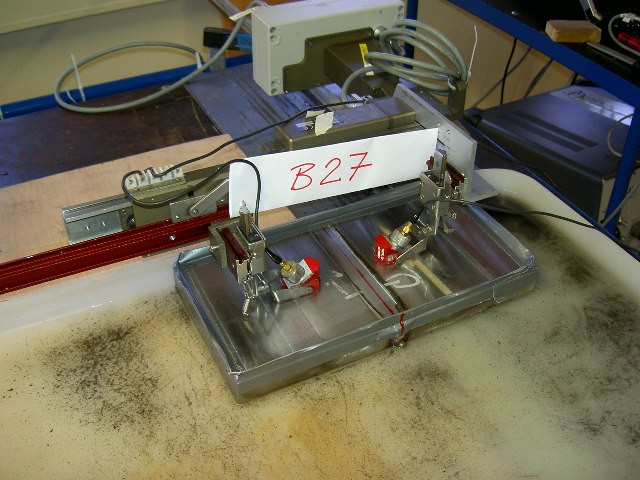
\includegraphics[height=5.84cm, width=7.78cm]{./figures/example-figure}
  \caption{Brief main caption. Essential details and comments may be given in this form after the caption. Capitalise only the first word of the caption and proper nouns contained within it.}\label{fig:my_label}
\end{figure}

\subsection{Tables}
Tables must be cited in the text and should be included as close to the point of reference as possible, but tables should not continue from one page to the next unless a table begins at the beginning of a page (ie, a multi-page table). The table caption, in bold and \(\SI{10}{\point}\), should always be centred with the table number above the table. Arabic numbers should be used for table numbers.

\begin{table}[H]
  \centering
  \caption{Table example}\label{tab:my_label}
  \begin{footnotesize}
    \begin{tabular}{p{6cm}p{8.7cm}}
      \hline
      Item                  & Specifications                                                                                                                                                                                                                        \\\hline
      Table caption defined & The table caption, in bold and Times New Roman \(\SI{10}{\point}\), should always be centred with the table number above the table.  Arabic numbers should be used for table numbers.  Do not end the table caption with a full stop. \\\hline
      Table contents        & Preferred type font is Times New Roman \(\SI{10}{\point}\).  Line spacing should be single space with one additional line of space between paragraphs.                                                                                \\\hline
    \end{tabular}
  \end{footnotesize}
\end{table}

\section{Conclusion}
Following the body of the report the author should present, in narrative format, conclusions drawn from the paper. The conclusions should be based on the discussion in the body of the paper. In addition, it may be valuable to demonstrate the value of the work to the profession. The conclusions should be written for the general reader. Specific detailed information is better confined to the body of the paper.

\section*{Acknowledgements}
Acknowledgements should be typed as text and placed before the reference listing.

\section*{References and footnotes}
References should be written in the order in which they appear in the text in the following format:

\printbibliography[heading=none]

The reference point in the text should be formatted thus~\cite{Tan1977}.\\

No footnotes will be shown at the bottom of pages.

\end{document}
